%************************************************
\chapter{Flourescence}
%************************************************
\begin{flushright}
November 1, 2012
\end{flushright}
\section{Objective}
To obtain a fluorescence spectrum of the fluorescence of the following kind
	\begin{enumerate}
		\item Constant incident frequency, varying detection frequency vs. Intensity detected
		\item Constant detection frequency (maxima), varying incident frequency vs. Intensity detected
		\item Varying concentration of solution, with both incident and detection frequencies fixed vs. Intensity detected
	\end{enumerate}

\section{Theory}
	Absorption works well when the concentration of the substance to be measured is high. When concentration gets smaller, the absorption gets noise prone and ceases to be reliable. With absorption we can get ppm, but with fluorescence, ppb is a routine affair. However it works IF the molecule fluoresces.
	\par
	Let's take a look at the fluorescence experiment. We start with a source of light which passes through a diffraction grating, excitation monochromater. Using this, a particular frequency of light is passed through the sample. Now perpendicular to it, there a detector, which comprises of a grating, viz. emission monochromater, and a photomultiplier. \marginpar{\Lisa The fluorescence is much smaller in intensity compared to the incident beam, thus perpendicular}
	\par
	Now before we continue, lets take a deeper look at what's happening. When an incident beam of light strikes a molecule, it goes from the ground electronic state to an excited electronic state. Now depending upon the frequency of the incident beam, the molecule will get into a vibrational state, while it's in the excited electronic state. The vibrational state quickly (within pico seconds typically) drops to the lowest vibrational state, since the molecule is in the liquid state. Consequently, regardless of the incident frequency (granted it's greater than the minimum required to excite the molecule to the first excited electronic state and less then the following electronic state), the molecule will drop from the lowest vibrational energy level in the excited electronic state, to the ground electronic state, at some vibrational state. Thus, if we obtain a graph between the frequency of light received and intensity, for a fixed incident frequency of light, we'll get a maxima corresponding to the ground vibrational state.
	Now if use the frequency for which we got the maximum intensity as constant, and change the incident beam's frequency, then again we'll get a maxima.
	If we use both these maxima values for the incident and emitted beam respectively, and change the concentration, we can use the obtained graph to find unknown concentrations.
	\par
	We must here realise that there's a phenomenon called Quenching that can kill the emission in fluorescence. Thus, we must perform a time resolved experiment, if a sample were to be analysed for further use.

\section{Observations/Discussion}
	The spectrum was not made available. The emission maxima was obtained at 512 nm, and the excitation maxima was obtained at 491 nm. Values for Concentration vs. Intenisty are given in \autoref{E6_int}. The graph is given in \autoref{E6_graph}
	\begin{table}
		\myfloatalign
		\begin{tabularx}{\textwidth}{Xll}
			\hline
			\tableheadline{Concentration (nano Molar)} 	&	\tableheadline{CPS} & \tableheadline{}\\				
			\hline%
			10.0 & 11070 & 0.2675\\
			5.0 & 39355 & 0.302\\
			2.5 & 14884 & 0.635\\		
			\hline%
		\end{tabularx}
		\caption{Concentration vs. Intensity}
		\label{E6_int}
	\end{table}

	\begin{figure}[bth]
		\begin{center}
			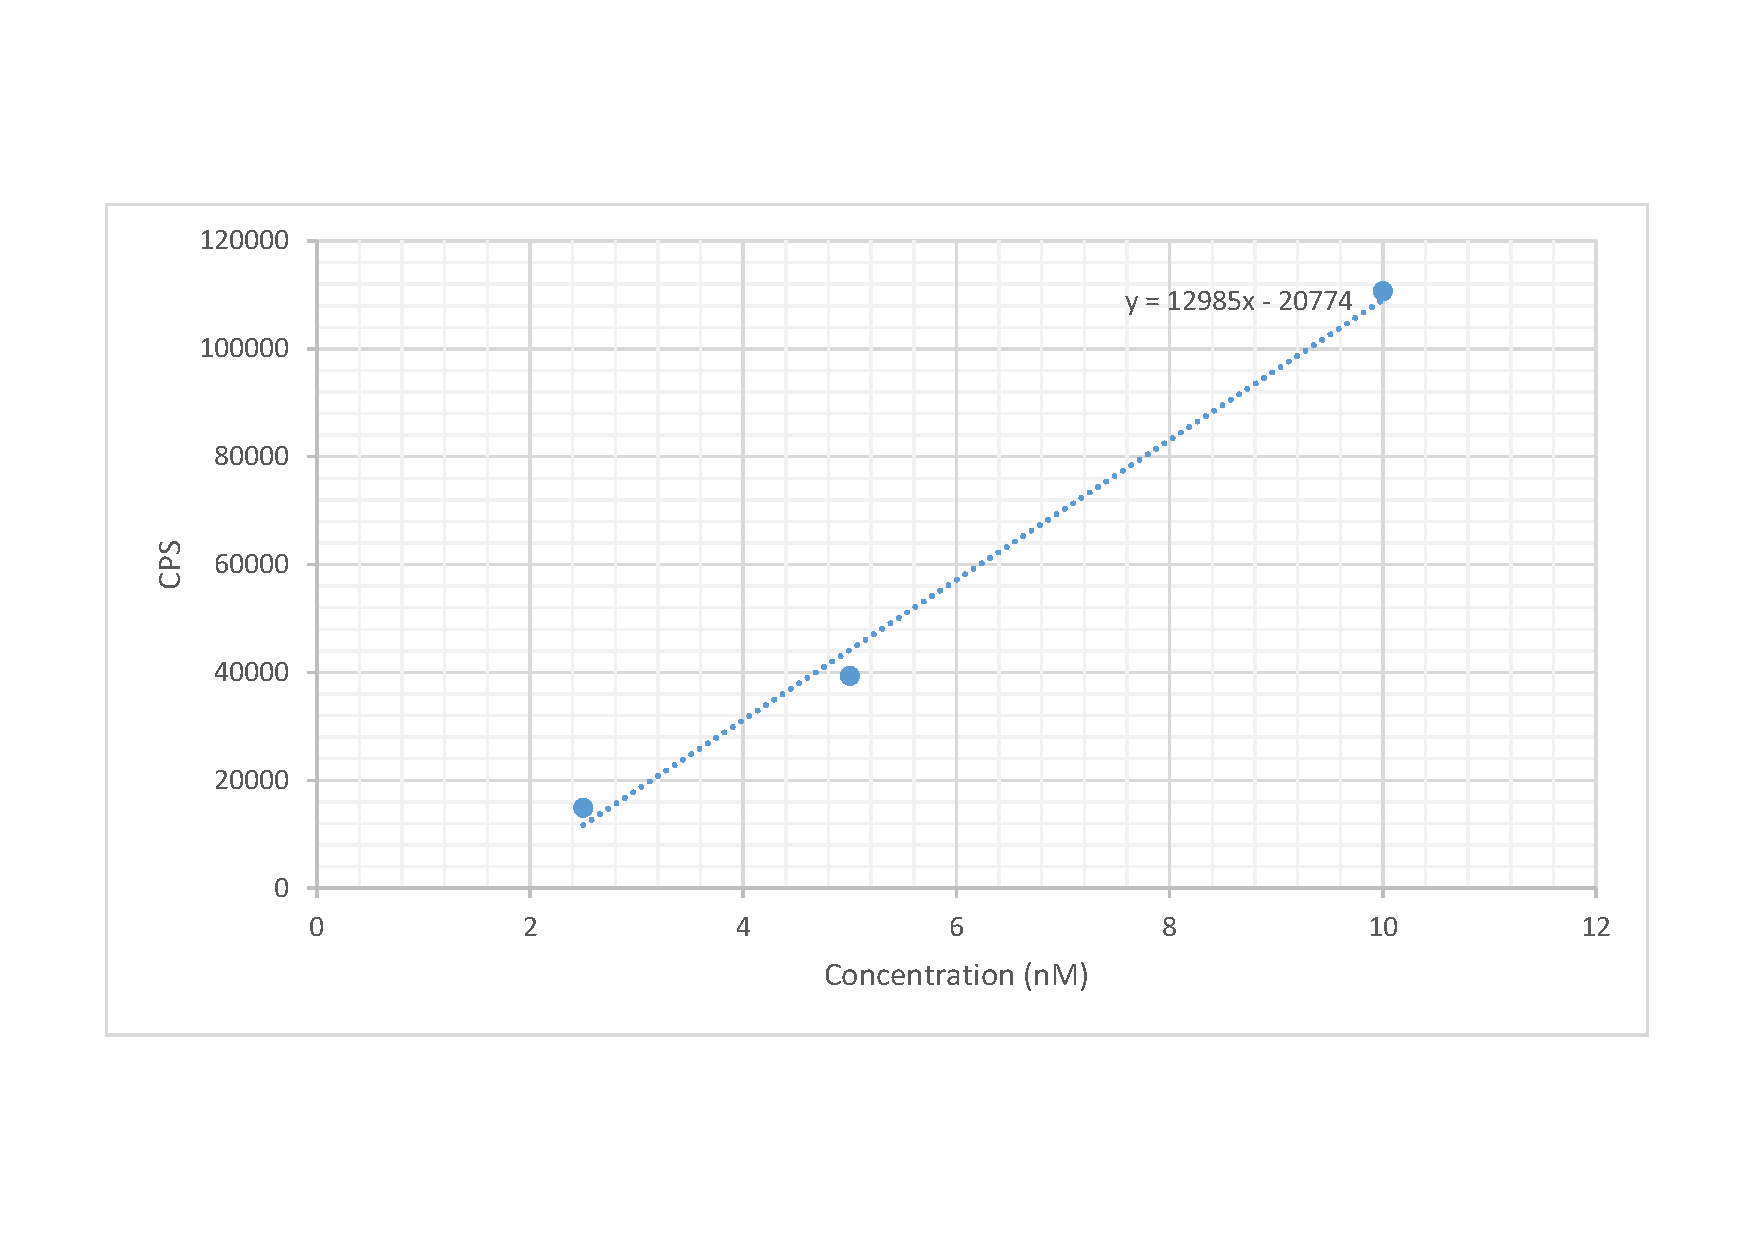
\includegraphics[width=1.15\linewidth]{gfx/6}
		\end{center}
	\caption[Concentration vs. Intensity]{\label{E6_graph}}
	\end{figure}

\section{Acknowledgements}
I thank our PhD assistant who performed the experiment for us, and of course Prof. KS Viswanathan for the rest.

\section{References}
	\begin{enumerate}
		\item Prof. K S Viswanathan's Lectures
	\end{enumerate}